\documentclass{svmono}
\usepackage[utf8]{inputenc}
\usepackage[T1]{fontenc}
\usepackage{lmodern}
\usepackage[portuguese,brazil]{babel}
\usepackage{hyperref}
\usepackage{enumerate}
\usepackage{amsmath,amssymb,amsfonts,mathptmx,helvet,courier,makeidx,graphicx,multicol}
\usepackage[bottom]{footmisc}
\usepackage{makeidx}

\newcommand{\Cdot}{\raisebox{-0.5ex}{\scalebox{2}{$\cdot$}}}
\newcommand{\hypersymb}{\#}
\newcommand{\hyper}[1]{{#1}^\hypersymb}

\newcommand{\dsfrac}[2]{\frac{\mbox{\normalsize\strut$#1$}}{\mbox{\normalsize\strut$#2$}}}
\newcommand{\dslim}[1]{\vphantom{\lim\limits_{\mathstrut{}#1}}\lim\limits_{#1}}
\newcommand{\vclear}[1]{\vphantom{\fbox{$#1$}}#1}

\newcommand{\Dy}{\Delta y}
\newcommand{\Dx}{\Delta x}
\newcommand{\Dz}{\Delta z}
\newcommand{\Du}{\Delta u}
\newcommand{\Dv}{\Delta v}
\newcommand{\Dt}{\Delta t}
\newcommand{\dy}{\dif y}
\newcommand{\dx}{\dif x}
\newcommand{\dz}{\dif z}
\newcommand{\du}{\dif u}
\newcommand{\dv}{\dif v}
\newcommand{\dt}{\dif t}

\newcolumntype{d}[1]{D{.}{,}{#1}}

\newcommand{\tnote}[1]{%
\footnote{N. do T.: #1}%
}

\newenvironment{caseanalysis}%
  {\par\indent\begin{enumerate}[\emph{Caso} \itshape1:]}%
  {\end{enumerate}}

\newenvironment{stepanalysis}%
  {\par\indent\begin{enumerate}[\emph{Passo} \itshape1:]}%
  {\end{enumerate}}

\newenvironment{enumeratewithspaces}[1][]%
  {\begingroup\setlength{\parskip}{1ex}\begin{enumerate}[#1]}%
  {\end{enumerate}\endgroup}%

% isto faz com que os contadores de exemplos e teoremas sejam
% reiniciados a cada seção
\makeatletter
\@addtoreset{theorem}{section}
\@addtoreset{example}{section}
\@addtoreset{corollary}{section}
\@addtoreset{lemma}{section}
\makeatother

% coloca o número da seção nas figuras
\usepackage{chngcntr}
\counterwithin{figure}{section}
\counterwithin{table}{section}
\counterwithin{equation}{section}
\renewcommand{\theequation}{\arabic{equation}}

%%%%%%%%%%%%%%%%%%%%%%%%%%%%%%%%%%%%%%%%%%%%%%%%%%%%%%%%%%%%%%%%%%
% commands to typeset the problem sections
% \exer - typeset one exercise
% \twoexer - typeset two exercises side by side
% \hardex - typeset a hard exercise
\newcounter{exerciseNo}

\newcommand{\exer}[1]{%

\begingroup%
\noindent\par%
\refstepcounter{exerciseNo}%
\begin{minipage}[t]{0.1\textwidth}%
\hspace{3ex}\textbf{\arabic{exerciseNo}}%
\end{minipage}%
\begin{minipage}[t]{0.9\textwidth}%
#1
\end{minipage}
\endgroup%

}

\newcommand{\twoexer}[2]{%

\begingroup%
\noindent\par%
\refstepcounter{exerciseNo}%
\begin{minipage}[t]{0.1\textwidth}
\hspace{3ex}\textbf{\arabic{exerciseNo}}
\end{minipage}%
\begin{minipage}[t]{0.4\textwidth}
#1
\end{minipage}%
\refstepcounter{exerciseNo}%
\begin{minipage}[t]{0.1\textwidth}
\hspace{3ex}\textbf{\arabic{exerciseNo}}
\end{minipage}%
\begin{minipage}[t]{0.4\textwidth}
#2
\end{minipage}
\endgroup%

}


\newcommand{\hardex}[1]{%

\noindent\par%
\begin{minipage}[t]{0.1\textwidth}
\begin{picture}(0,0)$\square$\end{picture}\hspace{3ex}\addtocounter{exerciseNo}{1}\textbf{\arabic{exerciseNo}}
\end{minipage}%
\begin{minipage}[t]{0.9\textwidth}
#1
\end{minipage}

}

%%%%%%%%%%%%%%%%%%%%%%%%%%%%%%%%%%%%%%%%%%%%%%%%%%%5
% sectionproblems environment

\newlength{\SectionProblemsSaveLengthA}
\newlength{\SectionProblemsSaveLengthB}

\newenvironment{sectionproblems}{%
  \setlength{\SectionProblemsSaveLengthA}{\parindent}
  \setlength{\SectionProblemsSaveLengthB}{\parskip}
  \setlength{\parindent}{0pt}
  \setlength{\parskip}{2pt}

  \section*{Problemas Para a Seção \the\value{chapter}.\the\value{section}}
  \setcounter{exerciseNo}{0}

}
{
  \setlength{\parindent}{\SectionProblemsSaveLengthA}
  \setlength{\parskip}{\SectionProblemsSaveLengthB}
}

%%%%%%%%%%%%%%%%%%%%%%%%%%%%%%%%%%%%%%%%%%%%%%%%%%%%%%%%%%%%%

\newenvironment{chapterproblems}
{
  \setlength{\SectionProblemsSaveLengthA}{\parindent}
  \setlength{\SectionProblemsSaveLengthB}{\parskip}
  \setlength{\parindent}{0pt}
  \setlength{\parskip}{2pt}

  \section*{Problemas Adicionais para o Capítulo~\the\value{chapter}}
  \sectionmark{Problemas Adicionais para o Capítulo~\the\value{chapter}}
  \addcontentsline{toc}{section}{Problemas Adicionais para o Capítulo~\the\value{chapter}}
  \setcounter{exerciseNo}{0}
}
{
  \setlength{\parindent}{\SectionProblemsSaveLengthA}
  \setlength{\parskip}{\SectionProblemsSaveLengthB}
}

\usepackage{ifthen}

\newcommand{\newdef}[2][]{%
\ifthenelse{\equal{#1}{}}%
{\textbf{#2}\index{#2}}%
{\textbf{#2}\index{#1}}%
}

\def\setR{\mathbb{R}}
\def\setHR{\hyper{\setR}}
\def\setN{\mathbb{N}}
\def\setZ{\mathbb{Z}}
\def\setQ{\mathbb{Q}}

\def\lth{\hyper{<}}
\def\definitionname{Definição}
\def\theoremname{Teorema}
\def\examplename{Exemplo}
\def\corollaryname{Corolário}
\def\lemmaname{Lema}
\spnewtheorem*{defin}{Definição}{\bfseries}{\rmfamily}
\spnewtheorem*{theor}{Teorema}{\bfseries}{\rmfamily}
\spnewtheorem*{warning}{Cuidado}{\bfseries}{\rmfamily}

\newtheorem*{lemma*}{Lema.}

\newcommand\subpart[1]{\paragraph{\textbf{#1}}}

% \narrowfigure[caption]{label}{commands}
\newcommand{\narrowfigure}[3][]{
\begin{figure}
#3
\caption{#1}
\label{#2}
\end{figure}
}

% \widefigure[caption]{label}{commands}
\newcommand{\widefigure}[3][]{
\narrowfigure[#1]{#2}{\begin{center}#3\end{center}}
}

% \narrowfigurefile[caption]{label}{path}
\newcommand{\narrowfigurefile}[3][]{
\narrowfigure[#1]{#2}{\includegraphics{#3}}
}

% \widefigurefile[caption]{label}{path}
\newcommand{\widefigurefile}[3][]{
\begin{figure}
\begin{center}
\includegraphics{#3}
\caption{#1}
\label{#2}
\end{center}
\end{figure}
}

%%%%%%%%%%%%%%%%%%%%%%%%%%%%%%%%%%%%%%%%%%%%%%%%%%%%%%%%%%%%%%%%

% \begin{includepic}[caption]{label}{width}{height}
%   this environment creates a picture environment inside a figure float
%   and defines a label fig:label. The picture dimensions are in mm.
\newenvironment{includepic}[3][]%
{
\begin{figure}
\begingroup
\def\thepiccaption{#1}
\def\thepiclabel{#2}
\setlength{\unitlength}{1mm}
\begin{center}
\begin{picture}(#3)
}
{
\end{picture}
\caption{\thepiccaption}
\label{fig:\thepiclabel}
\end{center}
\endgroup
\end{figure}
}


%%%%%%%%%%%%%%%%%%%%%%%%%%%%%%%%%%%%%%%%%%%%%%%%%%%%%%%%%%%%%%%%

% \includefig[caption]{filename}
%   this command creates a float, includes a picture from a file
%   and defines a label fig:filename
%   must have \graphicspath set beforehand
\newcommand{\includefig}[2][]{
\begin{figure}
\begin{center}
\includegraphics{#2}
\caption{#1}
\label{fig:#2}
\end{center}
\end{figure}
}

%%%%%%%%%%%%%%%%%%%%%%%%%%%%%%%%%%%%%%%%%%%%%%%%%%%%%%%%%%%%%%%%%%%

% \begin{includetable}[caption]{label}
%   this environment creates a table float and sets up tabular
%   spacing. A label tab:label will be created.
\newenvironment{includetable}[2][]%
{%
\begin{table}
\caption{#1}
\label{tab:#2}
\begingroup
\setlength{\tabcolsep}{1em}
\setlength{\extrarowheight}{2ex}
}%
{%
\endgroup
\end{table}
}

%%%%%%%%%%%%%%%%%%%%%%%%%%%%%%%%%%%%%%%%%%%%%%%%%%%%%%%%%%%%%%%%%%%%%%%
% \captions{left}{right}
% \includefigs{filenameleft}{filenameright}
%   these two commands define the captions, creates a float with
%   two pictures side by side and define the labels fig:filenameleft
%   and fig:filenameright
\def\TheLeftCaption{}
\def\TheRightCaption{}

\newcommand{\captions}[2]{
\def\TheLeftCaption{#1}
\def\TheRightCaption{#2}
}

\newsavebox{\IncludeFigLeftBox}
\newsavebox{\IncludeFigRightBox}

\newlength{\IncludeFigLeftBoxWidth}
\newlength{\IncludeFigRightBoxWidth}

\newcommand{\includefigs}[2]{
\savebox{\IncludeFigLeftBox}{\includegraphics{#1}}
\savebox{\IncludeFigRightBox}{\includegraphics{#2}}
\settowidth{\IncludeFigLeftBoxWidth}{\usebox{\IncludeFigLeftBox}}
\settowidth{\IncludeFigRightBoxWidth}{\usebox{\IncludeFigRightBox}}
\begin{figure}
\begin{minipage}[b]{\IncludeFigLeftBoxWidth}
\usebox{\IncludeFigLeftBox}
\caption{\TheLeftCaption}
\label{fig:#1}
\end{minipage}%
\hfill%
\begin{minipage}[b]{\IncludeFigRightBoxWidth}
\usebox{\IncludeFigRightBox}
\caption{\TheRightCaption}
\label{fig:#2}
\end{minipage}
\end{figure}
\def\TheLeftCaption{}
\def\TheRightCaption{}
}

%%%%%%%%%%%%%%%%%%%%%%%%%%%%%%%%%%%%%%%%%%%%%%%%%%%%%%%%%%%%%%%%%%%%%%

% \narrowtable[caption]{label}{coldef}{table}
\newcommand{\narrowtable}[4][]{
\begin{table}
\caption{#1}
\label{#2}
\begin{tabular}{#3}
#4
\end{tabular}
\end{table}
}

% \widetable[caption]{label}{coldef}{table}
\newcommand{\widetable}[4][]{
\begin{table}
\caption{#1}
\label{#2}
\begin{center}
\begin{tabular}{#3}
#4
\end{tabular}
\end{center}
\end{table}
}

\DeclareMathOperator{\std}{st}
\newcommand\Std[1]{\std\left(#1\right)}
\newcommand\st[1]{\std\left(#1\right)}

\def\endproof{\hfill$\blacksquare$}

\DeclareMathOperator{\sen}{sen}
\newcommand{\e}{e}

\def\SPC{\hspace{2ex}}

\newenvironment{interpretsolution}%
  {
    \begingroup
    \ifx\interpretsolutionbox\undefined
    \newsavebox\interpretsolutionbox
    \fi
    \sbox{\interpretsolutionbox}{\emph{Passo} \itshape3:{ }}
    \leftskip\wd\interpretsolutionbox\parindent0pt
    \hspace{-\wd\interpretsolutionbox}\emph{Interpretação da solução:} }%
  {\par\endgroup}

\spnewtheorem{contexample}{Exemplo}{\itshape}{\rmfamily}

\usepackage{refcount}

\newenvironment{examplecont}[1]%
{\setcounterref{contexample}{#1}\addtocounter{contexample}{-1}\begin{contexample}[continuação]}%
{\end{contexample}}

\newenvironment{absolutelynopagebreak}
  {\par\nobreak\vfil\penalty0\vfilneg
   \vtop\bgroup}
  {\par\xdef\tpd{\the\prevdepth}\egroup
   \prevdepth=\tpd}

\newenvironment{exsolution}
  {\noindent\emph{Solução:} }
  {}


\title{Cálculo Elementar}
\subtitle{Uma Abordagem por Infinitésimos}

\author{H. Jerome Keisler}

%%
% For nicely typeset tabular material
\usepackage{booktabs}

\makeindex

\begin{document}

\maketitle

% Front matter
\frontmatter

% r.1 blank page
\newpage

\setcounter{page}{3}

Dedicado a meus filhos, Randall, Jeffrey, e Thomas.

\hfill H. Jerome Keisler

\vfill

\emph{Haters gonna hate.}

\hfill Autor desconhecido

\vfill

Copyright © 2000 by H. Jerome Keisler.

Versão traduzida a partir da segunda edição americana, revista
em fevereiro de 2012. Traduzida em 2014 por Rodrigo Hausen.

Este trabalho está registrado sob a licença Creative Commons
por Atribuição-NãoComercial-CompartilhaIgual 3.0, de acordo
com o desejo original do autor. Para ver uma cópia desta licença,
visite \url{https://creativecommons.org/licenses/by-nc-sa/3.0/br/}
ou envie uma carta a Creative Commons, 559 Nathan
Abbott Way, Stanford, California, 93405, Estados Unidos.

\newpage

\chapter*{Prefácio à segunda edição americana}

Nesta segunda edição, várias mudanças foram feitas baseadas em nove
anos de experiência em sala de aula. Há revisões substanciais aos seis
primeiros capítulos e ao Epílogo, e há um capítulo completamente novo,
Capítulo 14, sobre equações diferenciais. Além disso, os Capítulos 11
e 12 originais foram reorganizados como três capítulos: Capítulo 11
sobre diferenciação parcial, Capítulo 12 sobre integração múltipla, e
Capítulo 13 sobre cálculo vetorial.

O Capítulo 1 foi encurtado, e a maior parte do material teórico da
primeira edição foi movida para o Epílogo. O cálculo de funções
transcendentais foi totalmente integrado ao curso, começando pelo
Capítulo 2 sobre derivadas. O Capítulo 3 foca em aplicações de
derivadas. O material sobre problemas com palavras e sobre taxas
relacionadas foi movido dos dois primeiros capítulos para o começo
do Capítulo 3. Os resultados teóricos sobre funções contínuas,
incluindo os Teoremas do Valor Intermediário, Extremo e Médio,
foram compilados em uma única seção ao final do Capítulo 2. O
desenvolvimenot da integral no Capítulo 4 foi simplificado. A 
%% TODO: "regra do trapézio"?
Regra do Trapézio foi trazida do Capítulo 5 para o Capítulo 4, e
uma discussão da Regra de Simpson foi adicionada. A seção sobre a
área entre duas curvas foi movida do Capítulo 4 para o Capítulo 4.
O Capítulo 5 lida com limites, aproximações e geometria analítica.
Um tratamento amplo às seções cônicas e uma seção sobre o método de
Newton foram adicionados. O Capítulo 6 começa com um novo material
sobre determinação de volume por integração de áreas de seções
transversais.

Apenas pequenas mudanças e correções foram feitas nos Capítulos 7
a 13. O novo Capítulo 14 fornece uma primeira introdução a equações
diferenciais, com ênfase na solução de equações diferenciais lineares
de primeira e segunda ordens. Na Seção 14.2, infinitésimos são usados
para dar uma prova simples à afirmação de que toda equação diferencial
$y' = f(t,y)$, onde $f$ é contínua, possui uma solução. A prova deste
fato está além do escopo de um curso de cálculo elementar, mas é alcançável
quando se usam infinitésimos.

Desejo agradecer todos os meus amigos e colegas que sugeriram correções
e aperfeiçoamentos à primeira edição deste livro. 

\hfill H. Jerome Keisler

\chapter*{Prefácio à primeira edição americana}

O cálculo foi originalmente desenvolvido usando-se o conceito intuitivo
de infinitésimo, ou um número infinitamente pequeno. Porém, nos últimos
cem anos, infinitésimos foram banidos do curso de cálculo por razões de
rigor matemático. Estudantes tiveram que aprender o assunto sem a
intuição original. Este livro de cálculo é baseado no trabalho de
Abraham Robinson, que em 1960 encontrou um modo de tratar com rigor os
infinitésimos. Enquanto que o curso tradicional começa com o conceito
difícil de limite, este curso inicia-se com infinitésimos, que são mais
fáceis de se compreender. Destina-se ao estudante médio que inicia em
cálculo e cobre a sequência usual de três ou quatro semestres.

A abordagem por infinitésimos tem três vantagens importantes para o
estudante. Primeiramente, é mais próxima da intuição que levou originalmente
ao cálculo. Em segundo lugar, os conceitos centrais de derivada e integral
tornam-se mais acessíveis a compreensão e uso pelo estudante. Por último,
ela ensina ambas as abordagens por infinitésimos e tradicional, dando ao
estudante uma ferramenta extra, a qual pode se tornar cada vez mais
importante no futuro.

Antes de descrever este livro, eu gostaria de inserir o trabalho de A.
Robinson no contexto histórico. Na década de 1670, Leibinitz e Newton
desenvolveram o cálculo com base na noção intuitiva de infinitésimos.
Os infinitésimos foram usados por mais duzentos anos, até que o
primeiro tratamento rigorozo do cálculo foi aperfeiçoado por
Weierstrass na década de 1870. O curso padrão de cálculo dos dias
de hoje ainda é baseado nas definições dadas por Weierstrass para o limite
``usando epsilons e deltas.'' Em 1960, Robinson resolveu um
problema de trezentos anos ao dar um tratamento preciso ao cálculo
usando infinitésimos. A conquista de Robinson provavelmente será
considerada um dos maiores avanços matemáticos do século XX.

Recentemente, infinitésimos tiveram empolgantes aplicações fora
da matemática, notadamente nos campos de economia e física. Como
é natural o uso de infinitésimos na modelagem de processos físicos
e sociais, tais aplicações certamente vão crescer em variedade
e importância. Esta é uma oportunidade única para encontrarmos
novos usos para a matemática, mas poucas pessoas foram atualmente
preparadas por meio de um treinamento que tire vantagem desta
oportunidade.

Sendo nova esta abordagem ao cálculo, alguns instrutores podem
precisar de materiais suplementares de apoio. Um volume do instrutor,
``\emph{Foundations of Infinitesimal Calculus}%
\tnote{Ainda não traduzido para o português.}%
,'' provê o suporte necessário e desenvolve a teoria em detalhe. O
volume do instrutor é atrelado a este livro, mas é autocontido
e destina-se ao público matemático geral.

Este livro contém todos os tópicos comuns de cálculo, incluindo a
definição tradicional de limite, além de uma ferramenta adicional
-- os infinitésimos. Assim, o estudante estará preparado para
cursos mais avançados da maneira que eles são ensinados atualmente.
Nos Capítulos de 1 até 4 os conceitos básicos de derivada, continuidade
e integral são desenvolvidos rapidamente pelo uso de infinitésimos. O
conceito tradicional de limite é adiado até o Capítulo 5, onde ele
é motivado por problemas de aproximação. Os últimos capítulos desenvolvem
funções transcendentais, séries, vetores, derivadas parciais e integrais
múltiplas. A teoria difere de um curso tradicional, mas a notação e os
métodos de solução de problemas são os mesmos na prática. Há uma variedade
de aplicações tanto a ciências naturais quanto sociais.

Eu incluí a seguinte inovação para instrutores que desejam introduzir
funções transcendentais cedo em seus cursos. No fim do Capítulo 2 sobre
derivadas, há um seção que começa um caminho alternativo sobre funções
transcendentais, e cada um dos Capítulos entre o 3 e o 6 possuem
caminhos alternativos com conjuntos de problemas sobre funções
transcendentais. Esta rota alternativa pode ser usada para fornecer
uma maior variedade nos problemas iniciais, ou pode ser omitida de
forma a se chegar às integrais o mais rápido possível. Nos Capítulos
7 e 8, as funções transcendentais são novamente desenvolvidas em um
ritmo mais lento.

Este livro é escrito para o estudante médio. Os problemas precedidos pelo
símbolo de um quadrado vão além dos exemplos trabalhados no texto e
destinam-se aos mais aventurosos.

Eu fui originalmente guiado a escrever este livro quando se tornou claro
para mim que o cálculo infinitesimal de Robinson poderia se tornar
disponível aos alunos de primeiro ano de um curso superior. A teoria é
apresentada de maneira simples; por exemplo, o trabalho de Robinson
usava lógica matemática, mas não este livro. Eu usei uma versão preliminar
deste livro em um curso de um semestre na Universidade de Wisconsin em
1969. Em 1971, foi publicada uma versão experimental para um curso em
dois semestres. Ela foi usada em várias faculdades e no colégio Nicolet,
próximo de Milwaukee, e foi testada em cinco escolas em um experimento
controlado, liderado pela Irmã Kathleen Sullivan entre 1972 e 1974. Os
resultados (publicados em 1974 na sua tese de doutoramento pela Universidade
do Wisconsin) mostram a viabilidade da abordagem por infinitésimos e serão
sumariados em um artigo no periódico American Mathematical Monthly\tnote{Sullivan, K. ``The Teaching of Elementary Calculus Using the Nonstandard Analysis Approach'', \emph{The American Mathematical Monthly}, v. 83, n. 5, 370--375, 1976.}.

Encontro-me em dívida com muitos colegas e estudantes que me encorajaram,
me deram conselhos e que cuidadosamente leram e usaram este manuscrito
em seus vários estágios de preparação. Devo agradecimentos especiais a
Jon Barwise, Universidade de Wisconsin; G. R. Blakley, Universidade de
Texas A \& M; Kenneth A. Bowen, Universidade de Syracuse; William P.
Francis, Universidade Tecnológica de Michigan; A. W. M. Glass,
Universidade de Bowling Green; Peter Loeb, Universidade de Illinois em
Urbana; Eugene Madison e Keith Stroyan, Faculdade Barat; e Frank Wattenberg,
Universidade de Massachusetts.

\hfill H. Jerome Keisler

\tableofcontents

\chapter*{Introdução}
\addcontentsline{toc}{chapter}{Introdução}

Enquanto a aritmética lida com somas, diferenças, produtos e quocientes, o
cálculo lida com derivadas e integrais. A derivada e a integral podem
ser descritas em linguagem comum em termos de uma viagem de carro. O
painel de instrumentos de um automóvel possui um \emph{velocímetro}
com marcações em quilômetros por hora e uma agulha que indica a velocidade.
O painel de instrumentos também tem um \emph{odômetro} que totaliza a
distância viajada em quilômetros (a quilometragem).

\vspace{0.5\baselineskip}
\begin{minipage}{0.5\textwidth}
\begin{center}
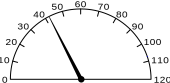
\includegraphics{figuras/introducao/velocimetro}\\
Velocímetro -- derivada da posição
\end{center}
\end{minipage}%
\begin{minipage}{0.5\textwidth}
\begin{center}
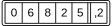
\includegraphics{figuras/introducao/odometro}\\
Odômetro -- integral da velocidade
\end{center}
\end{minipage}
\vspace{0.5\baselineskip}

Os valores indicados pelo velocímetro e pelo odômetro mudam com o tempo;
isto é, ambos são ``funções dependentes do tempo.'' A velocidade mostrada
no velocímetro é a taxa de variação, ou \emph{derivada}, da distância.
A velocidade é determinada tomando-se um intervalo de tempo muito
pequeno e calculando-se a razão entre a variação na distância e a
variação no tempo. A distância mostrada no odômetro é a
\emph{integral} da velocidade desde o instante inicial até o presente. 
A distância total é determinada pela adição das distâncias viajadas desde
o primeiro uso do carro até o presente.

O cálculo tem uma grande variedade de aplicações nas ciências naturais e
sociais. Algumas possibilidades estão ilustradas nos problemas.
Porém, é difícil prever futuras aplicações, portanto o próprio aluno
deve ser capaz de aplicar o cálculo a novas situações. Por esta razão, tão
importante quanto saber o que o cálculo pode fazer, é necessário aprender
por que ele funciona.
Para explicar por que o cálculo funciona, apresentaremos um grande número
de exemplos e desenvolveremos a teoria matemática com muito cuidado.

\mainmatter

\chapter{Números Reais e Hiper-reais}
\label{chp:reals}

O Capítulo~\ref{chp:reals} guia o estudante por um caminho direto até
o ponto onde será possível estudarmos derivadas. As Seções de%
~\ref{sec:realline} até \ref{sec:lines} apresentam uma revisão das
matérias que compõem o pré-cálculo e podem ser omitidas em muitos
cursos de cálculo. A Seção~\ref{sec:hyperrealline} fornece uma
explicação intuitiva para os números hiper-reais e como eles podem
ser usados para encontrar a inclinação de uma curva. Esta seção
não tem nenhum conjunto de problemas e destina-se a formar a base
de uma lição introdutória. O conteúdo principal do Capítulo~\ref{chp:reals}
está nas suas duas útimas seções, \ref{sec:infnumbers} e
\ref{sec:standardparts}. Nestas seções, o estudante aprenderá como
trabalhar com números hiper-reais e, em particular, como calcular
partes padrões. Partes padronizadas são usadas no início do próximo
capítulo para encontrar derivadas de funções. As Seções \ref{sec:infnumbers} e 
\ref{sec:standardparts} substituem os capítulos iniciais sobre limites,
encontrados nos textos tradicionais de cálculo.

Para o benefício do estudante interessado, incluímos um Epílogo ao final
do livro que apresenta a teoria por trás deste capítulo.

\section{A Reta Real}
\label{sec:realline}

A familiaridade com o sistema de números reais é um pré-requisito
para este curso. Uma revisão das regras da álgebra para números reais
é dada no apêndice. Por conveniência, estas regras estão também listadas
em uma tabela dentro da primeira capa deste livro. O símbolo
$\setR$ é usado para o conjunto de todos os números reais.
\tnote{Optamos por usar o negrito usado em lousa, ou dupla-cunhagem,
por ser mais familiar aos leitores brasileiros.}
Podemos pensar que os números reais estão dispostos ao longo de uma
reta, com os inteiros marcados a intervalos regulares, como na Figura%
~\ref{fig:realline}. Esta reta é chamada \newdef{reta real}.

\begin{figure}
\begin{center}
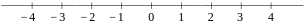
\includegraphics{figuras/chp_reals/realline}
\end{center}
\caption{A reta real.}
\label{fig:realline}
\end{figure}

Na matemática dos níveis fundamental e médio, a sistema de números
reais é construído gradualmente em vários estágios. Começando-se
pelos números naturais, continua-se com os inteiros,
racionais e, finalmente, os números reais são construídos. Uma
maneira de se construir o conjunto dos reais é defini-lo
como o conjunto de todos os números que possuem representação
decimal finita ou infinita após a vírgula.

Após a construção dos números reais, é possível demonstrar as
regras familiares de somas, diferenças, produtos, quocientes,
expoentes, raízes e ordem. Neste curso, assumiremos que estas
regras são familiares ao estudante, de tal forma que possamos
proceder o mais rápido possível para o cálculo.

Antes de continuarmos, faremos uma pausa para recapitular dois
pontos de especial importância ao cálculo. Em primeiro lugar,
\emph{a divisão por zero é proibida!} Expressões como
\[
\frac{2}{0}, \hspace{4ex} \frac{0}{0}, \hspace{4ex} \frac{x}{0} \hspace{4ex} \frac{5}{1+3-4}
\]
são sempre consideradas como \emph{indefinidas}.

Em segundo lugar, um número real positivo $c$ sempre possui duas
raízes quadradas, $\sqrt{c}$ e $-\sqrt{c}$, onde $\sqrt{c}$ sempre
representará a raiz quadrada positiva. Números reais negativos não
possuem raiz quadrada real. \emph{Para cada número real positivo
$c$, $\sqrt{c}$ é positivo e $\sqrt{-c}$ é indefinido.}

Por outro lado, cada número real possui apenas uma raiz cúbica real.
Se $c > 0$, então $c$ possui a raiz cúbica positiva $\sqrt[3]{c}$, e $-c$
possui a raiz cúbica negativa $\sqrt[3]{-c} = -\sqrt[3]{c}$.

No cálculo, geralmente lidamos com conjuntos de números reais. Por um
conjunto $C$ de números reais, queremos entender qualquer coleção de
números reais, chamados \emph{membros} de $C$, \emph{elementos} de $C$
ou \newdef{pontos} em $C$.

Um conjunto simples, mas importante, é um \newdef{intervalo}. Dados dois
números reais $a$ e $b$ tais que $a < b$, o
\newdef[intervalo!fechado]{intervalo fechado}
$[a,b]$ é definido como o conjunto de todos os números reais $x$
que satisfazem $a \le x$ e $x \le b$, ou de maneira mais concisa,
$a \le x \le b$.
O \newdef[intervalo!aberto]{intervalo aberto} $(a,b)$ é definido como o conjunto de todos
os números reais $x$ que satisfazem $a < x < b$. Intervalos fechados e
abertos estão ilustrados na Figura~\ref{fig:intervals}. 

\begin{figure}
\caption{}
\label{fig:intervals}
\end{figure}

Tanto para o intervalo aberto $(a,b)$, quanto para o intervalo
fechado $[a,b]$, o número $a$ é chamado de
\newdef[extremo!inferior]{extremo inferior},
e $b$ é o \newdef[extremo!superior]{extremo superior}. A diferença entre o
intervalo fechado $[a,b]$ e o intervalo aberto $(a,b)$ é que os extremos $a$
e $b$ são elementos de $[a,b]$, mas não elementos de $(a,b)$. Quando
$a \le x \le b$, dizemos que $x$ está \newdef{entre} $a$ e $b$; quando
$a < x < b$, dizemos que $x$ está \newdef{estritamente entre} $a$ e $b$.

Três outros tipos de conjuntos também são considerados intervalos
abertos: o conjunto $(a,\infty)$ dos números reais $x$ maiores do que $a$;
o conjunto $(-\infty,b)$ dos números reais $x$ menores do que $b$,
e toda a reta real $\setR$. A reta real $\setR$ é, às vezes, denotada
$(-\infty,\infty)$. Os símbolos $\infty$ e $-\infty$, lidos respectivamente
como ``infinito''  e ``menos infinito,'' não representam números reais; eles
só são usados, neste contexto, para indicar intervalos sem extremo
superior ou inferior.

Além dos intervalos fechados e abertos, há um outro tipo de intervalo,
chamado \newdef[intervalo!semiaberto]{intervalo semiaberto}. O conjunto
de todos os números
reais $x$ tais que $a \le x < b$ é um intervalo semiaberto denotado
$[a,b)$. O conjunto de todos os números reais $x$ tais que $a < x \le b$
é também um intervalo semiaberto denotado $(a,b]$.
A Tabela~\ref{tab:intervaltypes} mostra os vários tipos de intervalos.
\tnote{Nesta tradução, optamos por fazer correções sobre as classificações de intervalos neste parágrafo e na tabela.}

\begin{table}
\caption{Tipos de intervalos.}
\label{tab:intervaltypes}
\begin{center}
\begin{tabular}{l @{\hspace{3ex}} l @{\hspace{3ex}} l}
\hline
Tipo            & Símbolo         & Definição              \\
\hline
Fechado          & $[a,b]$         & $\{ x \in \setR | a \le x \le b \}$ \\
Fechado          & $[a,\infty)$    & $\{ x \in \setR | a \le x \}$ \\
Fechado          & $(-\infty,b]$   & $\{ x \in \setR | x \le b \}$ \\
Aberto           & $(a,b)$         & $\{ x \in \setR | a < x < b \}$ \\
Aberto           & $(a,\infty)$    & $\{ x \in \setR | a < x \}$ \\
Aberto           & $(-\infty,b)$   & $\{ x \in \setR | x < b \}$ \\
Semiaberto       & $(a,b]$         & $\{ x \in \setR | a < x \le b \}$ \\
Semiaberto       & $[a,b)$         & $\{ x \in \setR | a \le x < b \}$ \\
Fechado e aberto & $(-\infty,\infty)$ & $\setR$ \\
\end{tabular}
\end{center}
\end{table}

Listamos a seguir alguns outros conjuntos importantes de números reais.

\begin{enumerate}[(1)]
\item O conjunto vazio $\varnothing$, que não possui nenhum elemento.
\item O conjunto finito $\{ a_1, \ldots, a_n \}$, cujos únicos elementos
      são os números $a_1, a_2, \ldots, a_n$.
\item O conjunto $\setR^*$, ou seja, todo $x \in \setR$ tal que $x \ne 0$
\item O conjunto $\setN^* = \{ 1, 2, 3, 4, \ldots \}$ de todos os
      inteiros positivos%
\tnote{O autor usa apenas $\setN$ nesta definição. Optamos por usar
$\setN^*$ para evitar ambiguidade.}
\item O conjunto $\setZ = \{ \ldots, -3, -2, -1, 0, 1, 2, 3, \ldots \}$
      de todos os inteiros
\item O conjunto $\setQ$ de todos os números racionais. Um número
      racional é o quociente $m/n$ onde $m$ e $n$ são inteiros e $n \ne 0$.
\end{enumerate}

Enquanto que números reais correspondem a pontos em uma linha, pares
ordenados de números reais correspondem a pontos em um plano. Esta
correspondência nos dá uma maneira de desenhar gráficos de problemas
no cálculo, e de como traduzir problemas da física para a linguagem do
cálculo. É o ponto de partida da disciplina conhecida como
\newdef{geometria analítica}.

Um \newdef{par ordenado} de números reais, $( a,b )$, é dado
pelo primeiro número $a$ e pelo segundo número $b$. Por exemplo, $( 1,3 )$, $( 3,1 )$ e $( 1,1 )$ são três pares ordenados
diferentes. Seguindo a tradição, usaremos o mesmo símbolo para o intervalo
aberto $(a,b)$ e para o par ordenado $(a, b)$. Entretanto, o intervalo
aberto e o par ordenado são coisas compleramente diferente. Será sempre
óbvio pelo contexto se $(a,b)$ significa um intervalo aberto ou
um par ordenado.

Explicaremos como pares ordenados de números reais correspondem a
pontos no plano. Um sistema de \newdef{coordenadas retangulares} no
plano é dado por uma cópia horizontal e uma cópia vertical da reta
real, que se cruzam no zero. A reta horizontal é chamada \newdef{eixo
horizontal} ou \emph{eixo $x$}, enquanto que a reta vertical é chamada
\newdef{eixo vertical} ou \emph{eixo $y$}. O ponto onde os dois
eixos se encontram é chamado \emph{origem} e corresponde ao par
ordenado $(0,0)$. Considere agora um ponto qualquer $P$ no plano. Uma
reta vertical passando por $P$ cruzará o eixo $x$ em um número real
$x_0$, e uma reta horizontal por $P$ cruzará o eixo $y$ em um número
real $y_0$. O par ordenado $(x_0,y_0)$  obtido desta maneira corresponde
ao ponto $P$. (Ver Figura~\ref{fig:coordP}) Às vezes chamamos $P$ de ponto
$(x_0,y_0)$, e escreveremos $P(x_0,y_0)$. O número $x_0$ é dito
\newdef{coordenada $x$} de $P$, e $y_0$ é a \newdef{coordenada $y$} de $P$.

Por outro lado, dado um par ordenado $(x_0,y_0)$ de números reais, há um
ponto correspondente $P(x_0,y_0)$ no plano. Determinamos $P(x_0,y_0)$ pelo
ponto de interseção entre a reta vertical que cruza o eixo $x$ em $x_0$
e a reta horizontal que cruza o eixo $y$ em $y_0$. Descrevemos uma
correspondência biunívoca entre todos os pontos no plano e todos os
pares ordenados de números reais.

A partir de agora, simplificaremos as coisas por meio da identidade entre
pontos no plano e pares de números reais, conforme mostramos na Figura%
~\ref{fig:identidadepontos}.

\begin{figure}
\caption{}
\label{fig:coordP}
\end{figure}

\begin{figure}
\caption{}
\label{fig:identidadepontos}
\end{figure}

\begin{defin}
O \newdef{plano} $(x,y)$ é o conjunto de todos os pares ordenados $(x,y)$
de números reais. A \newdef{origem} é o ponto $(0,0)$. O \newdef{eixo $x$}
é o conjunto de todos os pontos na forma $(x,0)$, e o \newdef{eixo $y$} é
o conjunto de todo os pontos na forma $(0,y)$. 
\end{defin}

\section{Funções de Números Reais}
\label{sec:funcreal}

\section{Retas}
\label{sec:lines}

\section{Inclinação e Velocidade: a Reta Hiper-real}
\label{sec:hyperrealline}

\section{Números infinitesimais, finitos e infinitos}
\label{sec:infnumbers}

\subsection{O Princípio da Extensão}
\label{sec:extprinciple}

\subsection{O Princípio da Transferência}
\label{sec:transferprinciple}

\section{Partes Padronizadas}
\label{sec:standardparts}

\subsection{O Princípio da Parte Padronizada}
\label{sec:stpartprinciple}

\problemsection{\ref{chp:reals}}

\chapter*{Epílogo}
\addcontentsline{toc}{chapter}{Epílogo}

Como o cálculo por infinitésimos, da maneira como desenvolvido neste livro,
se relaciona com a abordagem tradicional para o cálculo, por meio de
épsilons e deltas ($\epsilon,\delta$)?
Para vermos as coisas pela perspectiva correta,
esboçaremos a história do cálculo.

Muitos problemas envolvendo inclinaçoes de retas, áreas e volumes, os quais
chamaríamos hoje de problemas de cálculo, foram resolvidos por antigos
matemáticos gregos. O maior de todos foi Arquimedes (287--212 A.C.).
Arquimedes antecipou tanto a abordagem por infinitésimos quanto a
abordagem por $\epsilon,\delta$. Por vezes, ele descobria seus resultados
através do raciocínio por infinitésimos, mas sempre publicava suas provas
usando o ``método da exaustão,'' que é similar à abordagem moderna por
$\epsilon,\delta$.

Problemas de cálculo tornaram-se importantes no início do século
XVII com o desenvolvimento da física e da astronomia. As regras
básicas de derivação e integração foram descobertas naquele período
por meio do raciocínio informal com infinitésimos. Kepler, Galileu,
Fermat e Barrow estiveram entre aqueles que contribuíram para esse
desenvolvimento.

Entre os anos de 1660 até o final da década de 1670, Sir Isaac Newton e
Gottfried Wilhelm Leibnitz ``inventaram'' independentemente o cálculo.
Eles deram o maior passo de reconhecer a importância de uma coleção
de resultados isolados e organizá-los em um todo.

Newton, em várias épocas, descreveu a derivada de $y$ (a qual ele
denominou ``fluxão\tnote{do original, ``fluxion.''}'' de $y$) de
três maneiras diferentes, em linhas gerais
\begin{enumerate}[(1)]
\item A razão entre uma mudança infinitesimal em $y$ em relação a
      uma mudança infinitesimal em $x$. (O método por infinitésimos.)
\item O limite da taxa de mudança em $y$ com relação à mudança em $x$,
      $\Delta y / \Delta x$, à medida que $\Delta x$ se aproxima de
      zero. (O método pelo limite.)
\item A velocidade de $y$ onde $x$ denota o tempo. (O método pela
      velocidade.)
\end{enumerate}

Em seus últimos escritos, Newton procurou evitar infinitesimais e
enfatizou os métodos (2) e (3). 

Leibiniz, por sua vez, consistentemente favorecia o método por infinitésimos,
mas acreditava (corretamente) que os mesmos resultados poderiam ser
obtidos usando-se apenas números reais. Ele considerava os infinitésimos
como números ``ideais,'' como os números imaginários. Para justificá-los,
ele propôs a lei da continuidade: ``Em qualquer transição suposta,
terminando em qualquer conclusão, é permissível instituir uma argumentação
geral, na qual a conclusão pode também ser incluída.''\footnote{Veja Kline, p. 385 e Boyer, p. 217} Esta ``lei'' é imprecisa demais para os padrões
atuais. Mas foi uma precursora notável do Princípio de Transferência
no qual o cálculo por infinitésimos moderno é baseado. Leibiniz estava
no caminho correto, mas chegou a ele 300 anos por demais cedo!

A notação desenvolvida por Leibinitz ainda está em uso geral nos dias de hoje,
mesmo tendo sido criada para sugerir o uso do método por infinitésimos:
$dy/dx$ para a derivada (para sugerir uma mudança infinitesimal em $y$
dividida por uma mudança infinitesimal em $x$), e $\int_b^a f(x) \mathrm{dx}$ para a integral (para sugerir a soma de uma quantidade infinita de
infinitésimos $f(x) \mathrm{dx}$).

Todas as três abordagens tinham sérias inconsistências, as quais foram
criticadas mais efetivamente por George Berkley\tnote{no original, ele
é denominado ``Bispo Berkley''} em 1734. Entretanto, um tratamento
preciso do cálculo estava além do estado da arte à época, e as
três descrições intuitivas da derivada (1)--(3) competiram entre si
pelos próximos duzentos anos. Até alguns anos após 1820,
o método infinitesimal (1) de Leibniz era o dominante no continente
europeu, por causa do seu apelo intuitivo e pela conveniência da
notação de Leibniz. Na Inglaterra, o método da velocidade (3)
predominava; ele também possui apelo intuitivo, mas não tem como
ser feito de maneira rigorosa.

Em 1821, A. L. Cauchy publicou um precursor do moderno tratamento para
o cálculo baseado no método pelo limite (2). Ele definiu tanto a integral
quanto a derivada em termos de limites, a saber
\[
\int_a^b f(x) \mathrm{dx} = \lim_{\Delta x \rightarrow 0^+} \sum_{a}^{b} f(x) \Delta x.
\]
Ele ainda usava infinitésimos, considerando-os como variáveis que
se aproximavam de zero. Daquele momento em diante, o método pelo
limite gradualmente se torno a abordagem predominante ao cálculom
enquanto que infinitésimos e apelos à velocidade sobreviveram apenas
como um modo de falar. Contudo, ainda havia dois pontos importantes a serem
tratados no trabalho de Cauchy. Primeiro, a definição de limite dada por
Cauchy não era suficientemente clasa; ainda dependia do uso intuitivo
de infinitésimos. Segundo, uma definição precisa do sistema de números
reais ainda não estava disponível. Tal definição precisaria de uma
melhor compreensão dos conceitos de conjunto e função, os quais ainda
estavam evoluindo.

Um tratamento completamente rigoroso do cálculo foi formulado finalmente
por Karl Weierstrass nos anos de 1870. Ele introduziu a condição
$\epsilon,\delta$ como a definição de limite. Aproximadamente nessa
época, alguns matemáticos (incluindo Weierstrass), foram bem sucedidos
na construção dos números reais a partir dos inteiros positivos. O
problema de construção do sistema de números reais também levou ao
desenvolvimento da teoria de conjuntos por Georg Cantor na mesma
década. A abordagem de Weierstrass tornou-se o tratamento tradicional,
ou ``padrão,'' para o cálculo como ele é apresentado hoje. Tudo começa
com a condição $\epsilon,\delta$ como a definição de limite e continua
com o desenvolvimento do cálculo apenas em termos do sistema de
números reais (sem mensão a infinitésimos). Entretanto, mesmo quando
o cálculo é apresentado na forma padrão, costuma-se argumentar
informalmente em termos de infinitésimos, e usa-se a notação de
Leibniz que sugere infinitésimos.

Desde os tempos de Weierstrass até muito recentemente, aparentava-se
que o método pelo limite (2) havia finalmente ganho a disputa e
que a história do cálculo elementar estava encerrada. Mas em 1934,
Thoralf Skolem construiu o que denominamos aqui por hiperinteiros,
e demonstrou que o análogo do Princípio da Transferência é válido para
eles. A construção de Skolem (agora chamada de construção pelo
ultraproduto) foi posteriormente estendida a uma grande classe de
estruturas, incluindo a construção dos números hiper-reais a partir
dos números reais. O nome ``hiper-real'' foi primeiramente usado por
E. Hewitt em um artigo de 1948. Os números hiper-reais eram conhecidos
mais de uma década antes de serem aplicados ao cálculo.

Finalmente, em 1960, Abraham Robinson descobriu que os números hiper-reais
poderiam ser usados para dar um tratamento rigoroso ao cálculo com
infinitésimos. A apresentação do cálculo dada neste livro é baseada
no tratamento de Robinson (mas modificada para torná-la adequada a um
primeiro curso).

O cálculo de Robinson segue o espírito do antigo método por infinitésimos
de Leibniz. Há grandes diferenças nos detalhes. Por exemplo, Leibniz
definiu a derivada como a razão $\Delta y / \Delta x$ onde $\Delta x$
é infinitesimal, enquanto que Robinson define a derivada como sendo
a \emph{parte padronizada} da razão $\Delta y / \Delta x$ onde $\Delta x$
é infinitesimal. Esta é a forma como Robinson evita as inconsistências
na abordagem antiga por infinitésimos. Além disso, a vaga lei da
continuidade de Leibniz é substituída pela formulação precisa do
Princípio da Transferência.

A razão pela qual o trabalho de Robinson não ter sido realizado antes é
que o Princípio da Transferência para números hiper-reais é um tipo de
axioms que não era familiar na matemática até recentemente. Ele emergiu
% TODO: verificar se model theory = teoria dos modelos
no campo da teoria dos modelos, que estuda a relação entre axiomas e
estruturas matemáticas. Os desenvolvimentos pioneiros na teoria dos
modelos não tinham sido feitos até os anos de 1930, por Gödel, Malcev,
Skolem e Tarski; o assunto mal existia até a década de 1950.

Olhando para trás, vemos que o método por infinitésimos era geralmente
o preferido, com relação ao método pelo limite, durante mais de 150 após
Newton e Leibniz terem inventado o cálculo, pois infinitésimos possuem
grande apelo intuitivo. Mas o método pelo limite foi finalmente adotado
ao redor de 1870 pois foi o primeiro tratamento matemático preciso para
o cálculo. Hoje em dia também é possível usar infinitésimos de uma
maneira matematicamente precisa. Os infinitésimos, no sentido proposto
por Robinson, tem sido aplicados não somente ao cálculo, mas também
ao campo mais amplo da análise. Eles levaram a novos resultados e
problemas em pesquisa matemática. Como os hiperinteiros de Skolem são
usualmente chamados de ``inteiros não padronizados,'' Robinson chamou
o novo campo de ``análise não padronizada.'' (Ele chamou os números
reais de ``padronizados'' e os demais números hiper-reais de
``não padronizados.'' Esta é a origem do nome ``parte padronizada.'')

O ponto de partida para este curso foi um par de descrições intuitivas
dos sistemas de números reais e hiper-reais. Essas descrições são,
na verdade, apenas esboços rudimentares que não são completamente
fiáveis. Para nos assegurarmos que os resultados estão corretos, o
cálculo deve ser baseado em descrições matematicamente precisas desses
sistemas de números, que preenchem as frestas nas descrições intuitivas.
Há dois modos de se fazê-lo. A maneira mais rápida é listar as propriedades
matemáticas dos números reais e hiper-reais. Estas propriedades devem ser
aceitas como básicas, e são chamadas \emph{axiomas}. A segunda maneira
de descrever matematicamente os números reais e hiper-reais é começar com
os inteiros positivos e, passo a passo, construir os inteiros, os 
números racionais, os números reais, e os números hiper-reais. Este
segundo método é melhor pois mostra que há realmente um estrutura com as
propriedades desejadas. No final deste epílogo, delinearemos brevemente a
construção dos números reais e hiper-reais e daremos alguns exemplos de
infinitésimos.

Nos dedicaremos, neste momento, à primeira maneira de descrever
matematicamente os números reais e hiper-reais. Listaremos dois grupos
de axiomas neste epílogo, um para números reais, e um para números
hiper-reais. Os axiomas para os números hiper-reais serão apenas
afirmações mais cuidadosas do Princípio da Extensão e do Princípio
da Transferência do Capítulo~\ref{chp:reals}. Os axiomas para os
números reais são apresentados em três partes: os Axiomas Algébricos, os
Axiomas de Ordem, e o Axioma da Completude. Todos os fatos familiares
sobre os números reais podem ser provados usando-se apenas estes
axiomas.

\subpart{I. Axiomas Algébricos dos Números Reais}

\begin{enumerate}[A]
\item Leis de fecho: $0$ e $1$ são números reais. Se $a$ e $b$ são
      números reais, também serão $a+b$, $ab$ e $-a$. Se $a$ é um
      número real e $a \ne 0$, então $1/a$ é um número real.
\item Leis de comutatividade: $a+b = b + a, \; \; ab = ba$
\item Leis de associatividade: $a+(b+c) = (a+b) + c, \; \; a(bc) = (ab)c$
\item Leis de identidade: $0 + a = a, \; \; 1 \cdot a = a.$
\item Leis de inversos: $a+(-a) = 0, \; \;$ Se $a \ne 0$, $a \cdot \frac{1}{a} = 1.$
\item Lei de distributividade: $a \cdot (b+c) = ab + ac.$
\end{enumerate}

\begin{defin}
Os \newdef{inteiros positivos} são os números reais $1$, $2 = 1+1$,
$3 = 1+1+1$, $4 = 1+1+1+1$ e daí em diante.
\end{defin}

\subpart{II. Axiomas de Ordem para Números Reais}

\begin{enumerate}[A]
\item $0 < 1$
\item Lei da transitividade: Se $a < b$ e $b < c$ então $a < c$.
\item Lei da tricotomia: Exatamente uma das relações $a < b$, $a = b$ ou $a > b$ é válida.
\item Lei da soma: Se $a < b$, então $a + c < b + c$.
\item Lei do produto: Se $a < b$ e $0 < c$, então $ac < bc$.
\item Axioma da raiz: Para todo número real $a > 0$ e todo inteiro positivo
      $m$, há um número real $b > 0$ tal que $b^n = a$.
\end{enumerate}

\subpart{III. Axioma da Completude}

Seja $A$ um conjunto de números reais tal que, toda vez que $x$ e $y$
estão em $A$, qualquer número real entre $x$ e $y$ também estará em $A$.
Então $A$ é um intervalo.

\begin{theor}
Uma sequência crescente $\langle S_n \rangle$ ou converge, ou diverge para
$\infty$.
\end{theor}

\begin{proof}
Seja $T$ o conjunto de todos os números reais $x$ tais que $x \le S_n$ para
algum $n$. Este conjunto é claramente não-vazio.

\begin{case}$T$ é toda a reta real. Se $H$ é infinito, temos que $x \le S_H$
para todo e qualquer número real $x$. Então $S_H$ é infinito positivo e
$\langle S_n \rangle$ diverge para $\infty$>
\end{case}

\begin{case}$T$ não é toda a reta real. Pelo Axioma de Completude,
$T$ é um intervalo $(-\infty,b]$ ou $(-\infty,b)$. Para todo número
real $x$ tal que $x < b$, temos
\[
	x \le S_n \le S_{n+1} \le S_{n+2} \le \ldots \le b
\]
para algum $n$. Disto decorre que, para um $H$ infinito, $S_H \le b$ e
$S_H \approx b$. Logo, $\langle S_n \rangle$ converge para $b$.
\end{case} \endproof%
\end{proof}

A partir de agora, atacaremos o segundo grupo de axiomas, os quais
fornecem as propriedades dos números hiper-reais. Haverá dois axiomas,
chamados Axioma da Extensão e Axioma da Transferência, que correspondem
ao Princípio da Extensão e ao Princípio da Transferência da Seção%
~\ref{sec:infnumbers}. Enunciaremos primeiro o Axioma da Extensão.

\subpart{I*. Axioma da Extensão}

\begin{enumerate}[(a)]
\item O conjunto $\setR$ dos números reais é um subconunto do conjunto
      $\setHR$ dos números hiper-reais.
\item Existe uma relação $\lth$ em $\setHR$, tal que:
      \begin{itemize}
      \item a relação de ordem $<$ em $\setR$ é a restrição de $\lth$
            aos reais;
      \item $\lth$ é transitiva ($a \lth b$ e $b \lth c$ implica $a \lth c)$; e
      \item $\lth$ satisfaz a Lei da Tricotomia (para quaisquer $a,b$ em $\setHR$, exatamente uma das afirmações $a \lth b$, $a = b$ ou $b \lth a$ é verdadeira).
      \end{itemize}
\item Existe um número hiper-real $\epsilon$ tal que $0 \lth \epsilon$ e
      $\epsilon \lth r$ para todo número real positivo $r$.
\item Para cada função real $f$, existe uma função hiperreal $\hyper{f}$
      com o mesmo número de variáveis, chamada \emph{extensão natural}
      de $f$ aos hiper-reais.
\end{enumerate}

A parte (c) do Axioma da Extensão afirma que há pelo menos um infinitésimo
positivo. A parte (d) nos dá a extensão natural para cada função real.
O Axioma da Transferência nos dirá que esta extensão natural possui as
mesmas propriedades da função original.

Lembre que o Princípio da Transferência da Seção~\ref{sec:infnumbers} fez
o uso da ideia intuitiva de uma afirmação sobre os reais. Antes de podermos
enunciar o Axioma da Transferência, devemos dar uma explicação matematicamente
precisa da noção de uma afirmação sobre os reais. Isto será feito em
vários passos, primeiro introduzindo-se os conceitos de uma expressão
real e de uma fórmula.

Começamos com o conceito de uma \newdef{expressão} real, ou \newdef{termo},
construído a partir de variáveis e constantes reais, usando funções reais.
Expressões reais podem ser construídas da seguinte forma:
\begin{enumerate}[(1)]
\item Uma constante real sozinha é uma expressão real.
\item Uma variável real sozinha é uma expressão real.
\item Se $e$ é uma expressão real, e $f$ é uma função real de uma variável,
      então $f(e)$ é uma expressão real. Similarmente, se $e_1, \ldots, e_n$
      são expressões reais e $g$ é uma função real de $n$ variáveis, então
      $g(e_1, \ldots, e_n)$ é uma expressão real.
\end{enumerate}

O passo (3) pode ser usado repetidamente para se construir expressões
mais longas. Alguns exemplos de expressões reais, onde $x$ e $y$ são
variáveis:
\[
2, \hspace{3ex} x+y, \hspace{3ex} |x-4|, \hspace{3ex} \sen(\pi y^2),
\hspace{3ex} \frac{\sqrt{x} + \sqrt{y}}{\sqrt{3}}, \hspace{3ex} g(x,f(0)),
\hspace{3ex} 1/0.
\]

Por \newdef{fórmula} queremos dizer uma afirmação de um dos tipos a seguir,
onde $d$, $e$ são expressões reais:
\begin{enumerate}[(1)]
\item uma \newdef{equação} entre duas expressões reais, $d = e$.
\item uma \newdef{inequação} entre duas expressões reais, $d < e$ ou
      $d \le e$ ou $d > e$ ou $d \ge e$ ou $d \ne e$.
\item uma afirmação na forma ``$e$ é definido'' ou ``$e$ é indefinido.''
\end{enumerate}
Eis aqui alguns exemplos de fórmulas:
\begin{eqnarray*}
  x + y & = & 5, \\
  f(x)  & = & \frac{1 - x^2}{1 + x}, \\
 g(x,y) & < & f(t), \\
 f(x,x) & \text{é} & \text{indefinido}.
\end{eqnarray*}
Se cada variável em uma fórmula for substituída por um número real, a
fórmula será ou verdadeira, ou falsa. Ordinariamente, a fórumula será
verdadeira para alguns valores de variáveis e falsa para outros. Por
exemplo, a fórmula $x+y = 5$ será verdadeira quando $(x,y) = (4,1)$
e falsa quando $(x,y) = (7,-2)$.

\begin{defin}
Uma \newdef{afirmação sobre os reais} é ou um conjunto finito e não vazio
de fórmulas $T$, ou uma combinação envolvendo dois conjuntos finitos e
não vazios de fórmulas $S$ e $T$ que afirma que ``sempre que todas as
fórmulas em $S$ forem verdadeiras, então todas as fórmulas em $T$ serão
verdadeiras.''
\end{defin}

Daremos vários comentários e exemplos para esclarecer esta definição. Por
vezes, ao invés de escrevermos ``sempre que todas as
fórmulas em $S$ forem verdadeiras, então todas as fórmulas em $T$ serão
verdadeiras'' usaremos a forma mais sucinta ``se $S$ então $T$'' para
uma afirmação sobre os reais. Cada um dos Axiomas Algébricos para os Números
Reais é uma afirmação sobre os reais. As leis da comutatividade,
associatividade, identidade e distributividade são afirmações sobre os
reais. Por exemplo, as leis da comutatividade são um par de fórmulas
\[
a  + b = b + a, \hspace{3ex} ab = ba,
\]
que envolvem duas variáveis $a$ e $b$. As leis de fecho podem ser expressas
como quatro afirmações sobre os reais:
\begin{eqnarray*}
a + b & \text{é} & \text{definido}, \\
ab    & \text{é} & \text{definido}, \\
-a    & \text{é} & \text{definido}, \\
\text{se } a \ne 0 \text{ então } 1/a & \text{é} & \text{definido}.
\end{eqnarray*}

\backmatter

\printindex

\end{document}
